\documentclass{article}
\usepackage{algorithms_in_data_mining}

\begin{document} %
\lecture{14}{Algorithms in Data Mining - Exam Answers}{Edo Liberty}

%\maketitle
\section*{General Info}
\begin{enumerate}
\item Solve $3$ out of $4$ questions.
\item Each correct answer is worth $35$ points and each part of a question $7$.
\item If you have solved more than three questions, please indicate which three you would like to be checked.
\item The exam's duration is 3 hours. If you need more time please ask the attending professor.
\item Good luck!
\end{enumerate}


\section*{Useful facts}
\begin{enumerate}
\item For any vector $x \in \R^{d}$ we define the $p$-norm of $x$ as
follows:
\[
||x||_p = [\sum_{i=1}^{d}(x(i))^p]^{1/p}
\]

\item {\bf Markov's inequality:} For any {\it non-negative} random variable
$X$:
\[
\Pr[X > t] \le E[X]/t.
\]
\item {\bf Chebyshev's inequality:} For any random variable $X$:
\[
\Pr[|X - E[X]| > t] \le \var[X]/t^2.
\]
\item {\bf Chernoff's inequality:} Let $x_1,\ldots,x_n$ be independent
$\{0,1\}$ valued random variables. Each $x_i$ takes the value $1$
with probability $p_i$ and $0$ else. Let $X = \sum_{i=1}^{n}x_i$ and
let $\mu = E[X] = \sum_{i=1}^{n}p_i$. Then:
\begin{eqnarray*}
\Pr[X > (1+\eps)\mu] &\le& e^{-\mu \eps^2/4}\\
\Pr[X < (1-\eps)\mu] &\le& e^{-\mu \eps^2/2}
\end{eqnarray*}
Or in a another convenient form:
\[
\Pr[|X - \mu| > \eps\mu] \le 2e^{-\mu \eps^2/4}
\]
%\item {\bf Hoeffding's inequality:} Let $x_1,\ldots,x_n$ be
%independent random variables taking values in $\{+1,-1\}$ each with
%probability $1/2$, then:
%\[
%\Pr[|\sum_{i=1}^{n}x_i a_i| > t] \le
%2e^{-\frac{t^2}{\sum_{i=1}^{n}a_{i}^{2}}}.
%\]
%\item For any $x \ge 2$ we have:
%\[
%e^{-1} \ge (1-\frac{1}{x})^{x} \ge \frac{2}{3}e^{-1}
%\]

%\item A probability distribution $\psi$ of $z$ is such that:
%\[
%\forall \; c_1,c_2 \in \R \;\; \Pr[c_1 \le z \le c_2]  = \int_{c_1}^{c_2}\psi(t)dt
%\]
%
%\item For a continuous variable $z$ we have that:
%\[%\begin{eqnarray*)
%\E[z] = \int_{-\infty}^{\infty} f(t)\psi(t)dt \;\;\;\;\;
%\Var[z] = \int_{-\infty}^{\infty} f^2(t)\psi(t)dt - (\E[z])^2
%\]%\end{eqnarray*}
\item $sin(0.005^{\circ}) \approx 9\cdot10^{-4} $, $cos(0.005^{\circ}) \approx 1 - 4\cdot10^{-7}$
\end{enumerate}

\pagebreak


%%%%%%%%%%%%%%%%%%%%%%%%%%%%%%%%%%%%%%%%%%%%%%%
%%%%%%%%%%%%%%%%%%%%%%%%%%%%%%%%%%%%%%%%%%%%%%%
%%%%%%%%%%%%%%%%%%%%%%%%%%%%%%%%%%%%%%%%%%%%%%%


\section{Probabilistic inequalities}
\subsection*{setup}
In this question you will be asked to derive the three most used
probabilistic inequalities for a specific random variable. Let
$x_1,\ldots,x_n$ be independent $\{-1,1\}$ valued random variables.
Each $x_i$ takes the value $1$ with probability $1/2$ and $-1$ else.
Let $X = \sum_{i=1}^{n}x_i$.

\subsection*{questions}
\begin{enumerate}
\item Let the random variable $Y$ be defined as $Y = |X|$.
Prove that Markov's inequality holds for $Y$. Hint: note that $Y$
takes integer values. Also, there is no need to compute $\Pr[Y =
i]$.
\item Prove Chebyshev's inequality for the above random variable
$X$. You can use the fact that Markov's inequality holds for any
positive variable regardless of your success (or lack of if) in the
previous question. Hint: $\var[X] = E[(X-E[X])^2]$.
\item Argue that
\[
\Pr[X > a] = \Pr[\Pi_{i=1}^{n}e^{\lambda x_i} > e^{\lambda a}] \le
\frac{E[\Pi_{i=1}^{n}e^{\lambda x_i}]}{e^{\lambda a}}
\]
for any $\lambda \in [0,1]$. Explain each transition.
\item Argue that:
\[
\frac{E[\Pi_{i=1}^{n}e^{\lambda x_i}]}{e^{\lambda a}} =
\frac{\Pi_{i=1}^{n}E[e^{\lambda x_i}]}{e^{\lambda a}} =
\frac{(E[e^{\lambda x_1}])^n}{e^{\lambda a}}
\]
What properties of the random variables $x_i$ did you use in each
transition?
\item Conclude that $\Pr[X > a] \le e^{-\frac{a^2}{2n}}$ by
showing that:
\[
\exists \;\;\lambda\in [0,1] \;\;s.t. \;\; \frac{(E[e^{\lambda
x_1}])^n}{e^{\lambda a}} \le e^{-\frac{a^2}{2n}}
\]
Hint: For the hyperbolic cosine function we have $\cosh(x) =
\frac{1}{2}(e^{x} + e^{-x}) \le e^{x^2/2}$ for $x \in [0,1]$.
\end{enumerate}
\pagebreak

%%%%%%%%%%%%%%%%%%%%%%%%%%%%%%%%%%%%%%%%%%%%%%%
%%%%%%%%%%%%%%%%%%%%%%%%%%%%%%%%%%%%%%%%%%%%%%%
%%%%%%%%%%%%%%%%%%%%%%%%%%%%%%%%%%%%%%%%%%%%%%%


\subsection*{answers}
\begin{enumerate}
\item 
\begin{eqnarray*}
E[Y] &=& \sum_{i=0}^{n}\Pr[Y=i]\cdot i\\
&=& \sum_{i=0}^{t}\Pr[Y=i]\cdot i + \sum_{i=t+1}^{n}\Pr[Y=i]\cdot i\\
&\ge& \sum_{i=t+1}^{n}\Pr[Y=i]\cdot i \\
&\ge& \sum_{i=t+1}^{n}\Pr[Y=i]\cdot t \\
&=& t\cdot\Pr[Y > t]
\end{eqnarray*}
Therefore, $E[Y] \ge t\cdot\Pr[Y > t]$ which is Markov's inequality.
\item This is identical to the general proof of Chebyshev's inequality.
We define $Z = (X - E[X])^2$. Since $Z$ is positive we can use Markov's inequality for it and get:
\[
\Pr[|X - E[X]| > t] = \Pr[Z > t^2] \le \frac{E[Z]}{t^2} = \frac{\var[X]}{t^2} 
\]
Here we used that $E[Z] = E[(X - E[X])^2] = \var[X]$.
\item First transition:
\[
\Pr[X > a] = \Pr[\lambda X > \lambda a] = \Pr[e^{\lambda X} > e^{\lambda a}] = \Pr[e^{\lambda \sum x_i} > e^{\lambda a}] = \Pr[\Pi_{i=1}^{n}e^{\lambda x_i} > e^{\lambda a}]
\]
These hold due to the monotonicity of multiplication by a positive constant and exponentiation.
Now, using Markov's inequality on the last inequality we get:
\[
\Pr[\Pi_{i=1}^{n}e^{\lambda x_i} > e^{\lambda a}] \le \frac{E[\Pi_{i=1}^{n}e^{\lambda x_i}]}{e^{\lambda a}} 
\]
\item The first transition is true due to the independence of the variables $x_i$. This means that $e^{\lambda x_i}$ are independent.
The second transition is due to all expectations of $e^{\lambda x_i}$ being equal which stems from $x_i$ being identically distributed.
\item First, we compute the expectation of $e^{\lambda x_i}$ 
\[
E[e^{\lambda x_i}] = \frac{1}{2}e^{\lambda} + \frac{1}{2}e^{-\lambda} = \cosh(\lambda) \le e^{\lambda^2/2}
\]
From the above we have that $\Pr[X > a] \le e^{n\lambda^2/2  - \lambda a}$. Setting $\lambda = a/n$ we get 
$e^{n\lambda^2/2  - \lambda a} = e^{-\frac{a^2}{2n}}$ which concludes the proof.
\end{enumerate}
\pagebreak



%%%%%%%%%%%%%%%%%%%%%%%%%%%%%%%%%%%%%%%%%%%%%%%
%%%%%%%%%%%%%%%%%%%%%%%%%%%%%%%%%%%%%%%%%%%%%%%
%%%%%%%%%%%%%%%%%%%%%%%%%%%%%%%%%%%%%%%%%%%%%%%




\section{Number of stars in the sky}
\subsection*{setup}
An enthusiast astronomer decides to count the number of stars in the sky (which are visible using her telescope).
She is rather low-tech so exact counting is out of the question. Alas, she knows that the visual angle of her telescope is $0.01^{\circ}$.
She figures out that this information should suffice in order to estimate the correct answer.
For simplicity, we assume she can point her telescope in any direction on the sphere, as if she is floating with her telescope in space.\footnote{This 
can actually be simulated by waiting for different parts of the day or year (you cannot look thorough the sun) but this discussion is irrelevant in this context.}
\begin{figure}[htbp]
\begin{center}
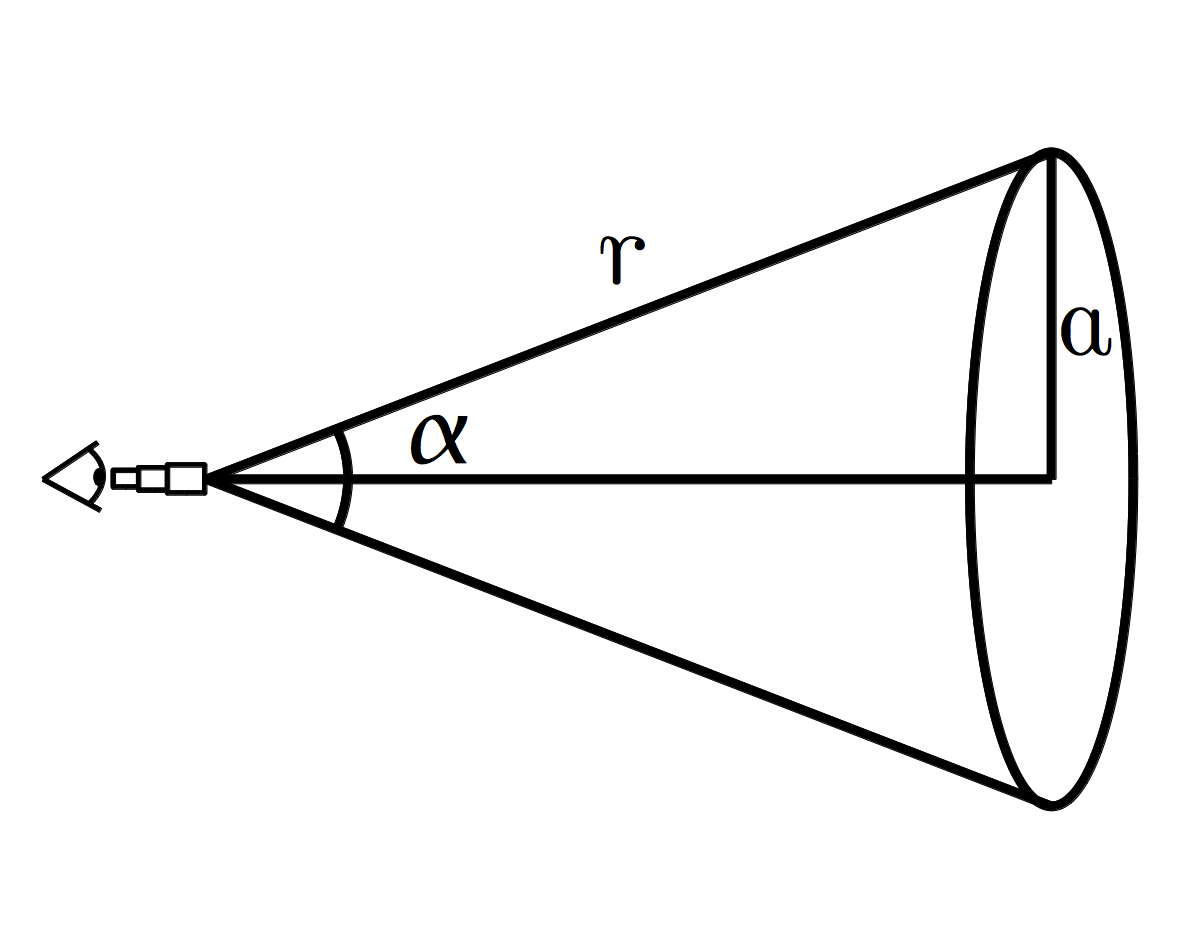
\includegraphics[scale=0.20]{14_images/Visual_angle.png}\hspace{3cm}
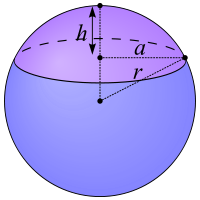
\includegraphics[scale=0.50]{14_images/Spherical_Cap.png}
\caption{On the left: an illustration of the visual angle $\alpha$ of a telescope ($sin(\alpha/2) = a/r$).
On the right: a spherical cap of base $a$ and height $h$ on a sphere of radius $r$. The area of the spherical cap is $2\pi r h$.
The surface area of the entire sphere is $4\pi r^2$.}
\label{default}
\end{center}
\end{figure}

\subsection*{questions}
\begin{enumerate}
\item What portion, $q$, of the sky does the telescope cover?
\item Let $x_i = 1$ if star $i$ is in the field of vision and zero else. 
If the telescope is pointed in a direction uniformly at random, what is the probability that $x_i = 1$.
You can use the quantity $q$ above even if you did not mange to solve the first question.
\item Denote by $N$ the number of visible stars. Let $z$ denote the number of visible stars, compute $\E[z]$.
\item Assume that one can never see more than $100Nq$ stars simultaneously through the telescope.
Show that $\Var[z] \le 100N^2q^2$
\item Define $Y = \frac{1}{s}\sum_{i=1}^{s}\frac{z_i}{q}$ where $z_i$ are independent star counts, each in an independent random direction. 
Compute a value for $s$ such that $\Pr[|Y - N| \ge \eps N] \le \delta$.
The value of $s$ should depend on both $\eps$ and $\delta$.
\end{enumerate}


%%%%%%%%%%%%%%%%%%%%%%%%%%%%%%%%%%%%%%%%%%%%%%%
%%%%%%%%%%%%%%%%%%%%%%%%%%%%%%%%%%%%%%%%%%%%%%%
%%%%%%%%%%%%%%%%%%%%%%%%%%%%%%%%%%%%%%%%%%%%%%%


\pagebreak
\subsection*{answers}
\begin{enumerate}
\item The portion of the sky the telescope covers is exactly the ratio between the area of the sphere $4\pi r^2$ and the area of the spherical cap $2\pi r h$ defined by the telescope. To compute $h$ we use simple trigonometry and get $h = r - r\cdot cos(0.005) = r \cdot 4\cdot10^{-7}$ (according to the attached useful information).
Finally $q = (2\pi r h)/(4\pi r^2) = 2\cdot10^{-7}$.
\item The probability that a star begin visible here is identical to the probability of it being visible in the scenario where the telescope is fixed and the star is located uniformly at random on the sphere.
In this scenario it is clear that the probability is exactly $q = 2\cdot10^{-7}$.
\item Note that $z = \sum_{i=1}^{n}x_i$. Computing the expectation:
$$
\E[z] = \E[\sum_{i=1}^{N}x_i] = \sum_{i=1}^{N} \E[x_i] = \sum_{i=1}^{N}q = Nq
$$
\end{enumerate}
\pagebreak



%%%%%%%%%%%%%%%%%%%%%%%%%%%%%%%%%%%%%%%%%%%%%%%
%%%%%%%%%%%%%%%%%%%%%%%%%%%%%%%%%%%%%%%%%%%%%%%
%%%%%%%%%%%%%%%%%%%%%%%%%%%%%%%%%%%%%%%%%%%%%%%

\section{Finding the number of users on Facebook}
\subsection*{setup}
Facebook does not publish exactly how many members it has. 
While the network does release official figures once in while there are good reasons to verify their reports.
One thing Facebook does offer is a web interface which allows external applications to receive information about specific users.
More specifically, given a user id the service returns some user data or not-a-user (if no such user exists).
This question will lead you through estimating the correct number of users using only this fact.
\subsection*{questions}
\begin{enumerate}
\item Assume that the number of users is $N$ and that user ids are $32$ bit integers.
If one picks a $32$ bit integer uniformly at random, what is the probability that it matches an existing user id. In other words, the returned response is not not-a-user.
\item Denote be $u(x)$ a function that takes the value $2^{32}$ if $x$ matches and existing user id and zero else.
Let $x_i$ be an integer drawn uniformly at random from $1,\ldots,2^{32}$. Compute the expected value of $$Z = \frac{1}{s}\sum_{i=1}^{s} u(x_i)$$
\item Show that the random variable $Y = 2^{-32}sZ$ is a sum of independent indicator $\{0,1\}$ variables.
\item Using the Chernoff bound, find a value for $s$ such that: $$\Pr[|Z-N| \ge \eps N] \le \delta$$ for given $\eps,\delta >0$.
\item Based on the fact that Facebook has more than $2^{29}$ users, would you consider this approach reasonable?
Lately, facebook changed their user id format to be a $64$ bit integer. Is this approach still reasonable?
\end{enumerate}

\pagebreak


%%%%%%%%%%%%%%%%%%%%%%%%%%%%%%%%%%%%%%%%%%%%%%%
%%%%%%%%%%%%%%%%%%%%%%%%%%%%%%%%%%%%%%%%%%%%%%%
%%%%%%%%%%%%%%%%%%%%%%%%%%%%%%%%%%%%%%%%%%%%%%%

\section{Simple high capacity hashing}
\subsection*{setup}
In this question we try to evaluate the capacity of a special hash table.
For simplicity, we assume that the hashed elements are a subset of $[N]$ ($[N]$ denotes the set $\{1,\dots,N\}$).
The hash table consists of an array $A$ of length $n$ and $L$ perfect hash functions $h_\ell: [N] \rightarrow [n]$.
Throughout the exercise we assume the existence of perfect hash functions. That is, $\Pr[h(x) = i] = 1/n$ for all $x \in [N]$ and $i\in [n]$ 
independently of the values $h(x')$.  For convenience we also assume that the entries in $A$ are initialized to the value $0$.
%
\begin{algorithm}
\caption{$Add(x)$}
\begin{algorithmic}
\FOR {$\ell \in [L]$}
    \IF {$A[h_\ell(x)] == 0$ or $A[h_\ell(x)] == x$}
    	\STATE $A[h_\ell(x)] = x$
	\STATE \RETURN Success
    \ENDIF
\ENDFOR
\STATE \RETURN Fail
\end{algorithmic}
\end{algorithm}
%
\vspace{-.6cm}
\begin{algorithm}
\caption{$Query(x)$}
\begin{algorithmic}
\FOR {$\ell \in [L]$}
    \IF {$A[h_\ell(x)] == x$}
	\STATE \RETURN True
   \ELSIF {$A[h_\ell(x)] == 0$}
   	\STATE \RETURN False
    \ENDIF
\ENDFOR
\STATE \RETURN False
\end{algorithmic}
\end{algorithm}
%
\vspace{-.6cm}
\subsection*{questions}
\begin{enumerate}
\item Argue the correctness of the hashing scheme. 
a) If an element was {\bf successfully} added to the table by $Add(x)$ it will be found by $Query(x)$. 
b) If an element was not added to the table by $Add(x)$ it will not be found by $Query(x)$. 
\item Assume that exactly $m$ cells in the array are occupied. That is, $m$ cells contain values $A[j] > 0$ and for the rest $A[j]=0$.
Given a new element $x$ which is in not stored in the hash table. What is the probability that location $h_1(x)$ in $A$ is occupied.
\item What is the probability that procedure $Add(x)$ fails for an element $x$ not in the hash table? (here we still assume there are exactly $m$ elements already in the table)
\item Assume we start with an empty hash table and insert $m$ elements one after the other. 
Use the union bound to get a value for $L$ for which $Add(x)$ succeeds in {\bf all} $m$ element insertions with probability at least $1-\delta$
\item Argue that the {\bf expected} running time of both $Add(x)$ and $Query(x)$ is $O(1)$. That is, it does not depend on $L$. 
\end{enumerate}


%%%%%%%%%%%%%%%%%%%%%%%%%%%%%%%%%%%%%%%%%%%%%%%
%%%%%%%%%%%%%%%%%%%%%%%%%%%%%%%%%%%%%%%%%%%%%%%
%%%%%%%%%%%%%%%%%%%%%%%%%%%%%%%%%%%%%%%%%%%%%%%

\end{document}
